\chapter{Theory}
\label{cha:theory}

In this section the theory behind the techniques used during the thesis work will be presented.
The first part will go through techniques used to process the data and perform an exploratory analysis.
After that text classifications, primarily with SVM, will be covered.
The last section contains an overview of the field of active learning, as well as a comparison of some different active learning techniques for multi-labeled data.

\section{Text Processing using Unsupervised Techniques}

Techniques in machine learning that does not require you have a categorized or labelled set of data is called unsupervised.
They use the structure of the data to obtain the information to use when processing it.
When it comes to text data, there are a few common methods and techniques that are unsupervised, and can be used for different purposes.
Examples of such techniques are \textit{topic modeling} and \textit{clustering}.
Another interesting technique is word2vec, that is used to produce word embeddings.

\subsection{Topic Modeling}

A topic model is a statistical model for finding topics within text~\cite{crain2012dimensionality}.
The topics build upon the probability that a certain word would occur in a text about a given topic, on the basis of terms occurring together.
For example, if the topic represents United States politics, words such as ``government'', ``Trump'', ``Reagan'', ``Senate'', or ``Medicaid'' are more likely to appear than ``sailboat'' or ``sweater''.
Any given document can then contain a topic with some probability.
This can be viewed as fuzzy clustering, and that the document has a degree of membership in a topic or cluster~\cite{crain2012dimensionality}.
The most common topic model in use is Latent Dirichlet Allocation (LDA)~\cite{crain2012dimensionality}.
Another topic model that preceded LDA is Probabilistic latent semantic analysis (PLSA)~\cite{hofmann1999probabilistic}.
However, PLSA has been shown to be more prone to overfitting than LDA~\cite{crain2012dimensionality}.

In the rest of the report, the following notation will be used:

\begin{itemize}
    \item D denotes a corpus of M documents: $D = \{w_1, w_2, \ldots, w_M\}$.
    \item The number of topics is $K$. Each topic is indexed by $i$.
    \item $N_d$ is the number of terms in document $d$.
    \item $N_i$ is the number of terms n topic $i$.
    \item $V$ denotes the number of words in the vocabulary.
\end{itemize}

\subsubsection{Latent Dirichlet Allocation}

Latent Dirichlet allocation (LDA) is a statistical model, where abstract topics in the model are defined as distributions over words~\cite{blei2003latent}.
LDA is based on a generative process, a model of which can be seen in Figure~\ref{fig:lda_gen_process}.
The circles in this figure represent random variables.
Dependencies between these random variables are shown with arrows, and if a variable is observed it is shaded in the figure.
In this model, the only observed variable is the words in the document.
Parts of the model are surrounded by a rectangle to show that the part is repeated several times.

\begin{figure}[!ht]
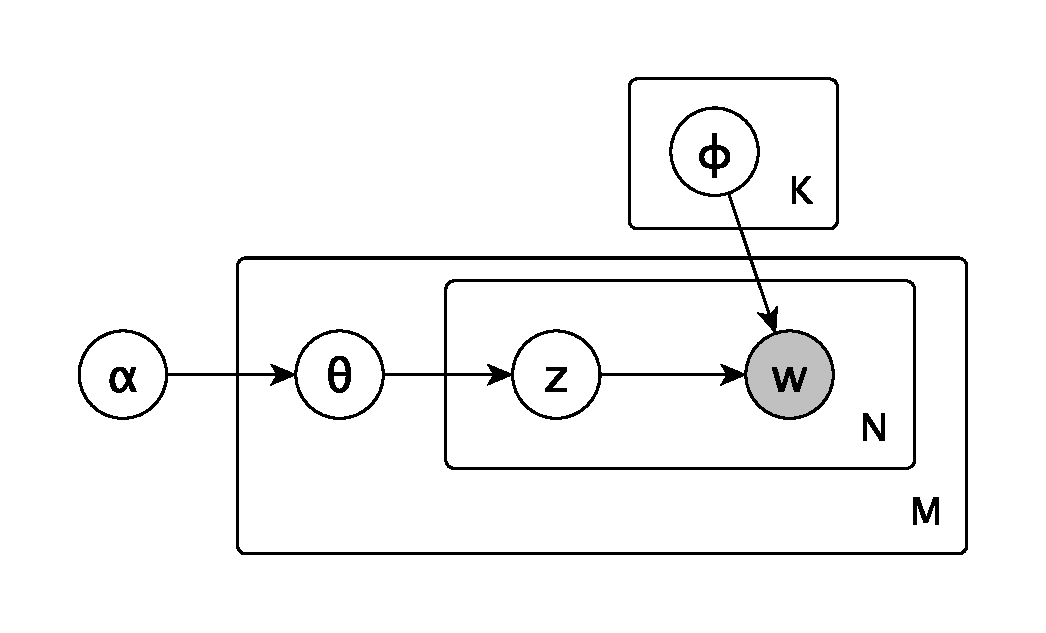
\includegraphics[scale=0.7]{figures/lda-generative-process.eps}
\caption{Diagram of the LDA model.}\label{fig:lda_gen_process}
\end{figure}

The generation of a corpus is done with the following steps~\cite{crain2012dimensionality, blei2003latent}:

\begin{itemize}
    \item \textbf{Draw a distribution over the words for each topic.}
        A sample $\phi_i$ is drawn from a symmetric Dirichlet distribution with parameter $\beta$. 
        This sample represents the distribution of terms for the topic $i$.

        \begin{equation}
            \Phi_i \sim Dir(\beta)
        \end{equation}

        \begin{equation}
            p(\Phi_i | \beta) = \frac{\Gamma(V\beta)}{{\Gamma(\beta)}^V} \prod^V_{v=1}\phi^{\beta-1}_{iv}
        \end{equation}

        Here, $\Gamma$ is the gamma function.

    \item \textbf{Draw a distribution over the topics for each document.}
        A sample $\theta_d$ is drawn from a Dirichlet distribution with parameters $\alpha$.
        This sample represents the distribution of topics for document $d$.

        \begin{equation}
            \Theta_d \sim Dir(\alpha)
        \end{equation}

        \begin{equation}
            p(\Theta_d | \alpha) = \frac{\Gamma(\sum^K_{i=1}\alpha_i)}{\prod_{i=1}^K\Gamma(\alpha_i)}\prod_{i=1}^K\theta_{di}^{\alpha_i-1}
        \end{equation}

    \item For each token with index n:

        \begin{itemize}
            \item \textbf{Draw a topic assignment $z_{dn}$ for the token index $n$.} 
                $z_{dn}$ is drawn from the distribution over topics for each document. 
                That is, $z_{dn}$ is drawn from a multinomial distribution using $\theta_d$ as a parameter.

                \begin{equation}
                    z_{dn} \sim Multinomial(\Theta_d)
                \end{equation}

                \begin{equation}
                    p(z_{dn} = i | \Theta_d) = \theta_{di}
                \end{equation}

            \item \textbf{Draw a token $w_{dn}$.}
                The token $w_{dn}$ is drawn from the topic distribution assigned to the index $n$.
                That is, $w_{dn}$ is drawn from a multinomial with parameter $\phi_{z_{dn}}$.

                \begin{equation}
                    w_{dn} \sim Multinomial(\Phi_{z_{dn}})
                \end{equation}

                \begin{equation}
                    p(w_{dn}=v|z_{dn}=i,\Phi_i) = \phi_{iv}
                \end{equation}

        \end{itemize}

\end{itemize}

The LDA model identifies topics from different terms that occur together.
Consider the case where an LDA model has been used to learn a number of topics.
Two terms that frequently occur together are then likely to be in the same topic.
So, if the same word has been used to express different thoughts, and the word has the same probability in two topics, the words that it co-occurs with can be used to differentiate between the different thoughts.

The task of learning the LDA model is a Bayesian Inference problem.
We have several variables that we cannot observe: the word distribution for the topics ($\phi_i$), the topic assignments for the tokens ($z$), and the topic distribution for the documents ($\theta_d$).
The only observed variables are the words in the document.
We have to approximate the posterior distribution using some sampling method, since it cannot be inferred automatically~\cite{blei2003latent}.

There exist a few algorithms that can be used to learn topics for the LDA model. 
Two of these that has shown to be able to extract useful topics from text are \textit{collapsed Gibbs sampling}~\cite{griffiths2004finding} and \textit{variational Bayes}~\cite{blei2003latent}.  
In collapsed Gibbs sampling, $\theta$ and $\phi$ are marginalized out.
It works by repeatedly sampling the topic assignment $z_{dn}$ for each token, conditioned on the assignments for the other tokens.
Variational Bayes works by using simpler single-variable models to approximate the LDA\@. 
As a consequence, it disregards any dependencies between the variables.
This is the approach used in the original LDA paper~\cite{blei2003latent}.

\subsubsection{Collapsed Gibbs}

% TODO: Write section on collapsed gibbs
\textit{To be written}

\subsection{Text Clustering}

Cluster analysis is commonly defined as finding groups in a given dataset.
The members of these groups are determined to be similar by a similarity measure~\cite{kaufman2009finding, aggarwal2012survey}.
Since text data is sparse, but yet have a very high dimensionality.
With one dimension per term in the dictionary, it is not uncommon with dimensions in the order of $10^5$.
For this reason, some of the more naive clustering algorithms does not work as well for text data~\cite{aggarwal2012survey}.

In distance-based clustering, a similarity function is used to measure the closeness between two text documents.
For the purpose of measuring the similarity between text objects, the cosine similarity function is most commonly used~\cite{aggarwal2012survey}.
Two different approaches to distance-based clustering are distance-based partitioning, and agglomerative hierarchical clustering.
%For distance-based clustering k-means and k-medoid are two the frequently used algorithms.
%When it comes to text data, k-means is preferred since k-medoid does not work as well for sparse data, and requires more iterations to converge~\cite{aggarwal2012survey}.

\subsubsection{K-means Clustering}

When using the k-means clustering algorithm, the clusters are based upon an initial set of k representatives.
A simple approach to k-means clustering can be seen as:

\begin{enumerate}
    \item Select K seeds from the original dataset
    \item \label{enum:k-means-step-2} Assign the rest of the documents to one of these seeds, based how how similar they are by the similarity function
    \item \label{enum:k-means-step-3} Before each new iteration, select a new centroid for each cluster. This should be the point that is the best central point for the cluster.
    \item Repeat step \ref{enum:k-means-step-2} and \ref{enum:k-means-step-3} until convergence.
\end{enumerate}

A visualization of this can be seen in Figure~\ref{fig:kmeans-iterations}.
One advantage that K-means has over K-medoid is that it requires a small number of iterations, especially compared to K-medoid~\cite{aggarwal2012survey, schutze1997projections}.
However, K-means is rather sensitive to the selection of initial seeds.
One approach is to just select them randomly, or selecting them based on the result of another lightweight clustering method.
A frequently used method is k-means++, that has been shown to improve both the speed and accuracy of k-means clustering~\cite{arthur2007k}.

\begin{figure}[h!]
    \centering
    \thirdsubfig{kmeans-init}{Initial seeds}
    \thirdsubfig{kmeans-iter1}{Iteration 1}
    \newline
    \thirdsubfig{kmeans-init2}{Centroids after iteration 1}
    \thirdsubfig{kmeans-iter2}{Iteration 2}
    \thirdsubfig{kmeans-init3}{Centroids after iteration 2}
    \caption{(a) to (e) shows iterations of K-means until convergence.
        In (e) it can be seen that the new centroids capture the same documents as the previous iteration, and we have converged.}
    \label{fig:kmeans-iterations}
\end{figure}

\subsubsection{Hierarchical Clustering}

% TODO: Write if needed
\textit{To be written if used in the end}

\section{Text Classification}

Text classification is a widely studied are within Computer Science.
It is an important problem in supervised machine learning, and it is task of assigning one or more classes to a given text document~\cite{aggarwal2012surveyclass}.
The problem is mainly approached with supervised machine learning.
That is, have a data set that consists of a collection of text documents, where each document has one or more classes assigned to it. % TODO: QUOTE BISHOP
This data set is then used to fit a classification model. 
The goal of this is for the model to be able to correctly assign a class to a a previously unseen text document.
Some of these classification models can also produce a probability of a document being of a certain class.
Other models are based on the concept of a margin that separates the classes, and the distance between a data point and a margin can be used to indicate how certain the model is of the assigned label~\cite{tong2001support}.
Example of use cases for text classification is categorization of news articles, document retrieval and email filtering.
There exists several different models for classifying text.
Decision trees, neural networks and Support Vector Machines (SVM) are some have been previously applied to the text domain with successful results~\cite{aggarwal2012survey}.
In this thesis, SVM are the main focus, since they have been studied extensively in the context of active learning. %TODO: CITE ALL OF THE SUPPORT VECTOR MACHINE ACTIVE LEARNING PAPERS

\subsection{Support Vector Machines}

SVMs work by implicitly map the training data to a feature space~\cite{bishop2006pattern}.
The goal is that the data should be linearly separable in the feature space, even if it is not in the input space.
In the case of binary classification, a point is classified by the linear model:

\begin{equation}
    y(x) = w^T \phi(x) + b
\end{equation}

The sign of $y(x)$ determines the label assigned to x.

SVMs work by trying to find the hyperplane that maximizes the margin.
That is, the distance between any point and the decision boundary should be as large as possible.
The hyperplane that gives us the maximum margin can be found by:

\begin{equation}
    \arg\min_{w,b}\frac{1}{2}||w||^2
\end{equation}

In order to allow for better generalization, and for data that isn't completely linearly separable, SVMs make use of slack variables $\xi_n$ to penalize points that are close to the decision boundary~\cite{bishop2006pattern}.
A parameter $C>0$ controls how much effect the slack variables will have.
The equation with the slack variables becomes:

\begin{equation}
    \arg\min_{w,b}\frac{1}{2}||w||^2 + C \sum_n\xi_n.
\end{equation}

A smaller $C$-value allows more points to be misclassified, in order to achieve better generalization.

\subsection{Multi-Label Classification}

Multi-label classification is the type of text classification where one instance can be associated with multiple labels.
It is a generalized version of the multi-class classification problem, where you have more than 2 labels, but each document is only assigned one.

A common way of solving multi-label classification problems is the binary Relevance method~\cite{read2011classifier}
It is a way of transforming the multi-label classification problem into several different binary ones.
With Binary Relevance you fit one classification model per label in your data.
Each of these classifiers are then predicting whether or not the document is associated with the corresponding label or not.

\section{Active Learning}

\subsection{Binary Minimization}

\subsection{MMC - Maximum Loss Reduction with Maximum Confidence}

\subsection{Adaptive Active Learning}